\documentclass{ximera}

%% You can put user macros here
%% However, you cannot make new environments

\listfiles

\graphicspath{{./}{firstExample/}{secondExample/}}

\usepackage{tikz}
\usepackage{tkz-euclide}
\usepackage{tikz-3dplot}
\usepackage{tikz-cd}
\usetikzlibrary{shapes.geometric}
\usetikzlibrary{arrows}
\usetikzlibrary{decorations.pathmorphing,patterns}
\usetkzobj{all}
\pgfplotsset{compat=1.13} % prevents compile error.

\renewcommand{\vec}[1]{\mathbf{#1}}
\newcommand{\RR}{\mathbb{R}}
\newcommand{\dfn}{\textit}
\newcommand{\dotp}{\cdot}
\newcommand{\id}{\text{id}}
\newcommand\norm[1]{\left\lVert#1\right\rVert}
 
\newtheorem{general}{Generalization}
\newtheorem{initprob}{Exploration Problem}

\tikzstyle geometryDiagrams=[ultra thick,color=blue!50!black]

\usepackage{mathtools}

\title{Constant Coefficient Homogeneous Systems I}%\label{Module 7-ADEF}


\begin{document}

\begin{abstract}

\end{abstract}

\maketitle

\section*{Constant Coefficient Homogeneous Systems I}

We'll now begin our study of the homogeneous system
\begin{equation}\label{eq:10.4.1}
{\bf y}'=A{\bf y},
\end{equation}
where $A$ is an $n\times n$ constant matrix. Since $A$ is continuous
on $(-\infty,\infty)$, Theorem~\ref{thmtype:10.2.1}
implies
that all solutions of \eqref{eq:10.4.1} are defined on $(-\infty,\infty)$.
Therefore, when we speak of solutions of ${\bf y}'=A{\bf y}$, we'll
mean solutions on $(-\infty,\infty)$.

In this section we assume that all the eigenvalues of $A$ are real and
that $A$ has a set of $n$ linearly independent eigenvectors. In the
next two sections we consider the cases where some of the eigenvalues
of $A$ are complex, or where $A$ does not have $n$ linearly
independent eigenvectors.

In Example~\ref{example:10.3.2} we showed that the vector
functions
$$
{\bf y}_1=\begin{bmatrix} -e^{2t}\\2e^{2t}\end{bmatrix}\quad\mbox{and}\quad
{\bf y}_2=\begin{bmatrix}-e^{-t}\\e^{-t}\end{bmatrix}
$$
form a fundamental set of solutions of the system
\begin{equation}\label{eq:10.4.2}
{\bf y}'=\begin{bmatrix}-4&-3\\6&5\end{bmatrix} {\bf y},
\end{equation}
but we did not show how we obtained ${\bf y}_1$ and ${\bf y}_2$ in the
first place. To see how these solutions can be obtained we write
\eqref{eq:10.4.2} as
\begin{equation}\label{eq:10.4.3}
\begin{array}{ccc}
y_1'&=&-4y_1-3y_2\\y_2'&=&6y_1+5y_2\end{array}
\end{equation}
and look for solutions of the form
\begin{equation}\label{eq:10.4.4}
y_1=x_1e^{\lambda t}\quad\mbox{and}\quad y_2=x_2e^{\lambda t},
\end{equation}
where $x_1$, $x_2$, and $\lambda$ are constants to be determined.
 Differentiating  \eqref{eq:10.4.4} yields
$$
y_1'=\lambda x_1e^{\lambda
t}\quad\mbox{ and }\quad y_2'=\lambda x_2e^{\lambda t}.
$$
Substituting this and  \eqref{eq:10.4.4} into  \eqref{eq:10.4.3} and canceling
the common factor $e^{\lambda t}$ yields
$$
\begin{array}{ccc}-4x_1-3x_2&=&\lambda x_1 \\
6 x_1+5x_2&=&\lambda x_2.\end{array}
$$
For a given $\lambda$, this is a homogeneous algebraic system, since it can
be rewritten as
\begin{equation}\label{eq:10.4.5}
\begin{array}{rcl} (-4-\lambda) x_1-3 x_2&=&0\\
6 x_1+(5-\lambda) x_2&=&0.\end{array}
\end{equation}
The trivial solution $x_1=x_2=0$ of this system isn't  useful, since
it corresponds to the trivial solution $y_1\equiv y_2\equiv0$ of
\eqref{eq:10.4.3}, which can't be part of a fundamental set of solutions
of \eqref{eq:10.4.2}. Therefore we consider only those values of $\lambda$
for which \eqref{eq:10.4.5} has nontrivial solutions. These are the values
of $\lambda$ for which the determinant of \eqref{eq:10.4.5} is zero;   that
is,
\begin{eqnarray*}
\begin{vmatrix}-4-\lambda&-3\\6&5-\lambda\end{vmatrix}&=&
(-4-\lambda)(5-\lambda)+18\\&=&\lambda^2-\lambda-2\\
&=&(\lambda-2)(\lambda+1)=0,
\end{eqnarray*}
which has the solutions $\lambda_1=2$ and $\lambda_2=-1$.

Taking $\lambda=2$ in  \eqref{eq:10.4.5} yields
\begin{eqnarray*}
-6 x_1-3 x_2&=&0\\
6 x_1+3 x_2&=&0,
\end{eqnarray*}
which implies that $x_1=-x_2/2$, where  $x_2$ can be
chosen arbitrarily. Choosing
$x_2=2$ yields the solution $y_1=-e^{2t}$,
$y_2=2e^{2t}$ of  \eqref{eq:10.4.3}. We can write this solution in vector
form as
\begin{equation}\label{eq:10.4.6}
{\bf y}_1=\begin{bmatrix} -1\\2\end{bmatrix} e^{2t}.
\end{equation}

Taking $\lambda=-1$ in  \eqref{eq:10.4.5} yields the system
\begin{eqnarray*}
-3 x_1-3 x_2&=&0\\
6 x_1+6 x_2&=&0,
\end{eqnarray*}
so $x_1=-x_2$. Taking $x_2=1$ here
yields the solution $y_1=-e^{-t}$, $y_2=e^{-t}$ of  \eqref{eq:10.4.3}. We
can write this solution in vector form as
\begin{equation}\label{eq:10.4.7}
{\bf y}_2=\begin{bmatrix}-1\\1\end{bmatrix}e^{-t}.
\end{equation}

In \eqref{eq:10.4.6} and \eqref{eq:10.4.7} the constant coefficients in the
arguments of the exponential functions are the eigenvalues of the
coefficient matrix in \eqref{eq:10.4.2}, and the vector coefficients of the
exponential functions are associated eigenvectors. This illustrates
the next theorem.

\begin{theorem}\label{thmtype:10.4.1}
 Suppose the $n\times n$
constant matrix $A$ has $n$ real eigenvalues
$\lambda_1,\lambda_2,\ldots,\lambda_n$
(which need not be distinct) with associated
linearly independent eigenvectors ${\bf x}_1,{\bf x}_2,\ldots,{\bf x}_n$.
Then the functions
$$
{\bf y}_1={\bf x}_1e^{\lambda_1 t},\,
 {\bf y}_2={\bf x}_2e^{\lambda_2 t},\,
\dots,\,
{\bf y}_n={\bf x}_ne^{\lambda_n t}
$$
 form a fundamental set of solutions of  ${\bf y}'=A{\bf y}$;
that is, the general solution of this system is
$$
{\bf y}=c_1{\bf x}_1e^{\lambda_1 t}+c_2{\bf x}_2e^{\lambda_2 t}
+\cdots+c_n{\bf x}_ne^{\lambda_n t}.
$$
\end{theorem}

\begin{proof}
Differentiating ${\bf y}_i={\bf x}_ie^{\lambda_it}$ and recalling
that $A{\bf x}_i=\lambda_i{\bf x}_i$ yields
$$
{\bf y}_i'=\lambda_i{\bf x}_ie^{\lambda_it}=A{\bf x}_ie^{\lambda_it}
=A{\bf y}_i.
$$
This shows that ${\bf y}_i$ is a solution of ${\bf y}'=A{\bf y}$.

The Wronskian of
 $\{{\bf y}_1,{\bf y}_2,\ldots,{\bf y}_n\}$ is
$$
\begin{vmatrix}  x_{11}e^{\lambda_1 t}& x_{12}e^{\lambda_2
t}&\cdots& x_{1n}e^{\lambda_n t}\\
 x_{21}e^{\lambda_1 t}& x_{22}e^{\lambda_2
t}&\cdots& x_{2n}e^{\lambda_n t}\\\vdots&\vdots&\ddots&\vdots\\
  x_{n1}e^{\lambda_1 t}& x_{n2}e^{\lambda_2
t}&\cdots& x_{nn}e^{\lambda x_n t}\end{vmatrix}
=e^{\lambda_1 t}e^{\lambda_2 t}\cdots e^{\lambda_n t}
\begin{vmatrix}
x_{11}&x_{12}&\cdots&x_{1n}\\
x_{21}&x_{22}&\cdots&x_{2n}\\
\vdots&\vdots&\ddots&\vdots\\
x_{n1}&x_{n2}&\cdots&x_{nn}
\end{vmatrix}.
$$
Since the columns of the determinant on the right are ${\bf x}_1, {\bf
x}_2, \dots, {\bf x}_n$, which are assumed to be linearly independent,
the determinant is nonzero. Therefore
Theorem~\ref{thmtype:10.3.3} implies that
$\{{\bf y}_1,{\bf y}_2,\ldots,{\bf y}_n\}$ is a fundamental set of
solutions of ${\bf y}'=A{\bf y}$.
\end{proof}

\begin{example}\label{example:10.4.1}

\begin{enumerate}
\item\label{item:10.4.1a} % (a)
 Find the general solution of
\begin{equation}\label{eq:10.4.8}
{\bf y}'=\begin{bmatrix}2&4\\4&2\end{bmatrix}
{\bf y}.
\end{equation}

\item\label{item:10.4.1b} % (b)
 Solve the initial value problem
\begin{equation}\label{eq:10.4.9}
{\bf y}'=\begin{bmatrix}2&4\\4&2\end{bmatrix}
{\bf y},\quad{\bf y}(0)=\begin{bmatrix}5 \\-1
\end{bmatrix}.
\end{equation}
\end{enumerate}

\begin{explanation}
\ref{item:10.4.1a}  The characteristic
polynomial of the  coefficient matrix $A$ in  \eqref{eq:10.4.8} is
\begin{eqnarray*}
\begin{vmatrix} 2-\lambda&4\\4&2-\lambda\end{vmatrix}
&=& (\lambda-2)^2-16\\
&=& (\lambda-2-4)(\lambda-2+4)\\
&=& (\lambda-6)(\lambda+2).
\end{eqnarray*}
Hence,  $\lambda_1=6$ and $\lambda_2
=-2$ are eigenvalues of $A$. To obtain the eigenvectors,
we must solve the system
\begin{equation}\label{eq:10.4.10}
\begin{bmatrix} 2-\lambda&4\\4&2-\lambda\end{bmatrix}
\begin{bmatrix} x_1\\x_2\end{bmatrix}=
\begin{bmatrix} 0\\0\end{bmatrix}
\end{equation}
with $\lambda=6$ and $\lambda=-2$.  Setting $\lambda=6$ in
\eqref{eq:10.4.10} yields
 $$
\begin{bmatrix}-4&4\\4&-4
\end{bmatrix}\begin{bmatrix}
x_1\\x_2\end{bmatrix}=\begin{bmatrix} 0\\0\end{bmatrix},
$$
which implies that $x_1=x_2$.  Taking $x_2=1$ yields the eigenvector
$$
{\bf x}_1=\begin{bmatrix} 1\\1\end{bmatrix},
$$
so
$$
{\bf y}_1=\begin{bmatrix} 1\\1\end{bmatrix}e^{6t}
$$
is a solution of  \eqref{eq:10.4.8}.  Setting $\lambda=-2$ in
\eqref{eq:10.4.10} yields
 $$
\begin{bmatrix} 4&4\\4&4\end{bmatrix}
\begin{bmatrix} x_1\\x_2
\end{bmatrix}=\begin{bmatrix} 0\\0\end{bmatrix},
$$
which implies that $x_1=-x_2$.  Taking $x_2=1$ yields the eigenvector
$$
{\bf x}_2=\begin{bmatrix}-1\\1\end{bmatrix},
$$
so
$$
{\bf y}_2=\begin{bmatrix}-1\\1\end{bmatrix}e^{-2t}
$$
is a solution of  \eqref{eq:10.4.8}.
From Theorem~\ref{thmtype:10.4.1}, the general solution of
\eqref{eq:10.4.8} is
\begin{equation}\label{eq:10.4.11}
{\bf y}=c_1{\bf y}_1+c_2{\bf y}_2=c_1\begin{bmatrix}1\\1
\end{bmatrix}e^{6t}+c_2\begin{bmatrix}-1\\1
\end{bmatrix}e^{-2t}.
\end{equation}


\ref{item:10.4.1b}
 To satisfy the initial condition in  \eqref{eq:10.4.9}, we must choose
$c_1$ and $c_2$ in  \eqref{eq:10.4.11} so that
$$
c_1\begin{bmatrix}1\\1\end{bmatrix}+c_2\begin{bmatrix}-1\\
1\end{bmatrix}=\begin{bmatrix}5\\-1
\end{bmatrix}.
$$
This is equivalent to the system
\begin{eqnarray*}
c_1-c_2&=&5\\
c_1+c_2&=&-1,
\end{eqnarray*}
so $c_1=2, c_2=-3$.  Therefore the solution of
\eqref{eq:10.4.9} is
$$
{\bf y}=2\begin{bmatrix}1\\1\end{bmatrix}e^{6t}-3
\begin{bmatrix}-1\\1\end{bmatrix}e^{-2t},
$$
or, in terms of components,
$$
y_1=2e^{6t}+3e^{-2t},\quad y_2=2e^{6t}-3e^{-2t}.
$$
\end{explanation}
\end{example}

\begin{example}\label{example:10.4.2}

\begin{enumerate}
\item\label{item:10.4.2a} % (a)
 Find the general solution of
\begin{equation}\label{eq:10.4.12}
{\bf y}'=\begin{bmatrix}3&-1&-1\\-2&
3&
2\\4&-1&-2\end{bmatrix}{\bf y}.
\end{equation}

\item\label{item:10.4.2b}  % (b)
 Solve the initial value problem
\begin{equation}\label{eq:10.4.13}
{\bf y}'=\begin{bmatrix}3&-1&-1\\-2&3&
2\\4&-1&-2\end{bmatrix}{\bf y},\quad{\bf y}(0)=\begin{bmatrix}2\\
-1\\8\end{bmatrix}.
\end{equation}
\end{enumerate}


\begin{explanation}   
\ref{item:10.4.2a} The characteristic
polynomial of the  coefficient matrix $A$ in  \eqref{eq:10.4.12} is
$$
\begin{vmatrix}3-\lambda&-1&-1\\-2&3-\lambda&
2\\4
&-1&-2-\lambda\end{vmatrix}=-(\lambda-2)(\lambda-3)(\lambda+1).
$$
Hence, the eigenvalues of $A$ are $\lambda_1=2$, $\lambda_2=3$,  and
$\lambda_3=-1$.
To find the  eigenvectors, we must solve the system
\begin{equation}\label{eq:10.4.14}
\begin{bmatrix}3-\lambda&-1&-1\\-2&3-\lambda&
2\\4&-1&
-2-\lambda\end{bmatrix}\begin{bmatrix} x_1\\x_2\\x_3
\end{bmatrix}=\begin{bmatrix}0\\0\\0\end{bmatrix}
\end{equation}
with $\lambda=2$, $3$, $-1$.  With $\lambda=2$, the augmented matrix of
\eqref{eq:10.4.14} is
$$
\begin{bmatrix} 1&-1&-1&\vdots&0\\-2&
1&2&\vdots&0\\4&-1&-4&\vdots&0
\end{bmatrix},
$$
which is row equivalent to
$$
\begin{bmatrix} 1&0&-1&\vdots&0\\0&1&0&
\vdots&0\\0&0&0&\vdots&0\end{bmatrix}.
$$
Hence,  $x_1=x_3$ and $x_2=0$.  Taking $x_3=1$ yields
$$
{\bf y}_1=\begin{bmatrix}1\\0\\1\end{bmatrix}e^{2t}
$$
as a solution of  \eqref{eq:10.4.12}.  With $\lambda=3$, the augmented
matrix of  \eqref{eq:10.4.14} is
$$
\begin{bmatrix}0&-1&-1&\vdots&0\\-2&
0& 2&\vdots&0\\4&-1&-5&\vdots&0
\end{bmatrix},
$$
which is row equivalent to
$$
\begin{bmatrix} 1&0&-1&\vdots&0\\0&1&1&
\vdots&0\\0&0&0&\vdots&0\end{bmatrix}.
$$
Hence,  $x_1=x_3$ and $x_2=-x_3$. Taking $x_3=1$ yields
$$
{\bf y}_2=\begin{bmatrix}1\\-1\\1\end{bmatrix}e^{3t}
$$
as a solution of  \eqref{eq:10.4.12}.  With $\lambda=-1$, the augmented
matrix of  \eqref{eq:10.4.14} is
$$
\begin{bmatrix} 4&-1&-1&\vdots&0\\-2&4&
2&\vdots&0\\4&-1&-1&\vdots&0
\end{bmatrix},
$$
which is row equivalent to
$$
\begin{bmatrix} 1&0&-1/7&\vdots&0\\0&1&
3/7&\vdots&0\\0&0&0&\vdots&0\end{bmatrix}.
$$
Hence, $x_1=x_3/7$ and $x_2=-3x_3/7$.  Taking $x_3=7$ yields
$$
{\bf y}_3=\begin{bmatrix}1\\-3\\7\end{bmatrix}e^{-t}
$$
as a solution of  \eqref{eq:10.4.12}. By Theorem~\ref{thmtype:10.4.1},
 the general solution of  \eqref{eq:10.4.12} is
$$
{\bf y}=c_1\begin{bmatrix}1\\0\\1\end{bmatrix}e^{2t}
+c_2\begin{bmatrix}1\\-1\\1\end{bmatrix}
e^{3t}+c_3
\begin{bmatrix}1\\-3\\7\end{bmatrix}e^{-t},
$$
which can also be written as
\begin{equation}\label{eq:10.4.15}
{\bf y}=\begin{bmatrix}e^{2t}&e^{3t}&e^{-t}
\\0&-e^{3t}&
-3e^{-t}\\e^{2t}&e^{3t}&7e^{-t}\end{bmatrix}\begin{bmatrix} c_1\\c_2\\c_3\end{bmatrix}.
\end{equation}

\ref{item:10.4.2b}
 To satisfy the initial condition in  \eqref{eq:10.4.13} we must choose
$c_1$, $c_2$, $c_3$ in  \eqref{eq:10.4.15} so that
$$
\begin{bmatrix}1&1&1\\0&-1&-3\\
1&1&7\end{bmatrix}
\begin{bmatrix} c_1\\c_2\\c_3\end{bmatrix}=
\begin{bmatrix}2\\-1\\8\end{bmatrix}.
$$
Solving this system yields $c_1=3$, $c_2=-2$, $c_3=1$.  Hence, the solution
of  \eqref{eq:10.4.13} is
\begin{eqnarray*}
{\bf y}&=&\begin{bmatrix}e^{2t}&e^{3t}&
e^{-t}\\0&-e^{3t}
&-3e^{-t}\\e^{2t}&e^{3t}&7e^{-t}\end{bmatrix}
\begin{bmatrix}3\\-2\\1\end{bmatrix}\\
&=&3\begin{bmatrix}1\\0\\1\end{bmatrix}e^{2t}-2
\begin{bmatrix}1\\-1\\1\end{bmatrix}
e^{3t}+\begin{bmatrix}1\\-3\\7\end{bmatrix}e^{-t}.
\end{eqnarray*}
\end{explanation}
\end{example}

\begin{example}\label{example:10.4.3}
 Find the general solution of
\begin{equation}\label{eq:10.4.16}
{\bf y}'=\begin{bmatrix}-3&2&2\\
2&-3&2\\2&2&-3
\end{bmatrix}{\bf y}.
\end{equation}


\begin{explanation} The characteristic polynomial of
the  coefficient matrix $A$ in  \eqref{eq:10.4.16} is
$$
\begin{vmatrix}-3-\lambda&2&2\\2&-3-\lambda&2\\2&2
&-3-\lambda\end{vmatrix}=-(\lambda-1)(\lambda+5)^2.
$$
Hence, $\lambda_1=1$ is an eigenvalue of multiplicity $1$, while
$\lambda_2=-5$ is an eigenvalue of multiplicity $2$. Eigenvectors
associated with $\lambda_1=1$ are solutions of the system with
augmented matrix
$$
\begin{bmatrix}-4&2&2&\vdots&0\\
2
&-4&2&\vdots&0\\2&2&-4&
\vdots&0\end{bmatrix}, $$
which is row equivalent to
$$
\begin{bmatrix} 1&0&-1&\vdots& 0\\0&1&-1 &\vdots& 0
\\0&0&0&\vdots&0\end{bmatrix}.
$$
Hence, $x_1=x_2=x_3$, and we choose $x_3=1$ to obtain the solution
\begin{equation}\label{eq:10.4.17}
{\bf y}_1=\begin{bmatrix}1\\1\\1\end{bmatrix}e^t
\end{equation}
of  \eqref{eq:10.4.16}.  Eigenvectors associated with $\lambda_2=-5$
are solutions of the system
with  augmented matrix
$$
\begin{bmatrix} 2&2&2&\vdots&0\\2&2&2&\vdots&0
\\2&2&2&\vdots&0\end{bmatrix}.
$$
Hence, the components of these eigenvectors need only satisfy the single
condition
$$
x_1+x_2+x_3=0.
$$
Since there's only one equation here, we can choose $x_2$ and
$x_3$  arbitrarily. We obtain one eigenvector by choosing $x_2=0$
and $x_3=1$, and another by choosing $x_2=1$ and $x_3=0$. In both
cases $x_1=-1$. Therefore
$$
\begin{bmatrix}-1\\0\\1\end{bmatrix}\quad
\mbox{and}\quad\begin{bmatrix}-1\\1\\0
\end{bmatrix}
$$
are linearly independent eigenvectors associated with  $\lambda_2=
-5$, and the corresponding solutions of  \eqref{eq:10.4.16} are
$$
{\bf y}_2=\begin{bmatrix}-1\\0\\1\end{bmatrix}e^{-5t}\quad
\mbox{and}\quad{\bf y}_3=\begin{bmatrix}-1\\1\\
0\end{bmatrix}e^{-5t}.
$$
Because of this and  \eqref{eq:10.4.17}, Theorem~\ref{thmtype:10.4.1} implies
that  the general solution of \eqref{eq:10.4.16} is
$$
{\bf y}=c_1\begin{bmatrix}1\\1\\
1\end{bmatrix}e^t+c_2
\begin{bmatrix}-1\\0\\1\end{bmatrix}
e^{-5t}+c_3\begin{bmatrix}-1\\1\\0\end{bmatrix}e^{-5t}.
 $$

\end{explanation}
\end{example}

\subsection*{Geometric Properties of Solutions when  $n=2$}

We'll now  consider the geometric properties of solutions of a
$2\times2$ constant coefficient system
\begin{equation} \label{eq:10.4.18}
\begin{bmatrix}y_1'\\y_2'\end{bmatrix}=\begin{bmatrix}a_{11}&a_{12}\\a_{21}&a_{22}
\end{bmatrix}\begin{bmatrix}y_1\\y_2\end{bmatrix}.
\end{equation}
It is convenient to think of a ``$y_1$-$y_2$ plane," where a point
is identified by rectangular coordinates $(y_1,y_2)$. If ${\bf
y}=\begin{bmatrix}y_1\\y_2\end{bmatrix}$ is a non-constant solution of \eqref{eq:10.4.18},
then the point $(y_1(t),y_2(t))$ moves along a curve $C$ in the
$y_1$-$y_2$ plane as $t$ varies from $-\infty$ to $\infty$. We call
$C$ the \dfn{trajectory} of ${\bf y}$. (We also say that $C$ is a
trajectory of the system \eqref{eq:10.4.18}.) It's important to note that
$C$ is the trajectory of infinitely many solutions of \eqref{eq:10.4.18},
since if $\tau$ is any real number, then ${\bf y}(t-\tau)$ is a
solution of \eqref{eq:10.4.18} %(Exercise~\ref{exer:10.4.28}(b)), 
and
$(y_1(t-\tau),y_2(t-\tau))$ also moves along $C$ as $t$ varies from
$-\infty$ to $\infty$. Moreover, Exercise~\ref{exer:10.4.28}%\part{c}
implies
that distinct trajectories of \eqref{eq:10.4.18} can't intersect, and that
two solutions ${\bf y}_1$ and ${\bf y}_2$ of \eqref{eq:10.4.18} have the
same trajectory if and only if ${\bf y}_2(t)={\bf y}_1(t-\tau)$ for
some $\tau$.

From Exercise~\ref{exer:10.4.28}%\part{a}, 
a trajectory of a nontrivial
solution
of \eqref{eq:10.4.18} can't contain $(0,0)$, which we define to be the
trajectory of the trivial solution ${\bf y}\equiv0$. More generally,
if ${\bf y}=\begin{bmatrix}k_1\\k_2\end{bmatrix}\neq{\bf 0}$ is a constant solution
of \eqref{eq:10.4.18} (which could occur if zero is an eigenvalue of the
matrix of \eqref{eq:10.4.18}), we define the trajectory of ${\bf y}$ to be
the single point $(k_1,k_2)$.

To be specific, this is the question: What do the trajectories look
like, and how are they traversed? In this section we'll answer this
question, assuming that the matrix
$$
A=\begin{bmatrix}a_{11}&a_{12}\\a_{21}&a_{22}
\end{bmatrix}
$$
of \eqref{eq:10.4.18} has real eigenvalues $\lambda_1$ and $\lambda_2$ with
associated linearly independent eigenvectors ${\bf x}_1$ and ${\bf
x}_2$. Then  the general solution of \eqref{eq:10.4.18} is
\begin{equation} \label{eq:10.4.19}
{\bf y}= c_1{\bf x}_1
 e^{\lambda_1 t}+c_2{\bf x}_2e^{\lambda_2 t}.
\end{equation}
We'll consider other situations in the next two sections.

We leave it to you %(Exercise~\ref{exer:10.4.35}) 
to classify the
trajectories of \eqref{eq:10.4.18} if zero is an eigenvalue of $A$. We'll
confine our attention here to the case where both eigenvalues are
nonzero. In this case the simplest situation is where
$\lambda_1=\lambda_2\neq 0$, so  \eqref{eq:10.4.19} becomes
$$
{\bf y}=(c_1{\bf x}_1+c_2{\bf x}_2)e^{\lambda_1 t}.
$$
Since ${\bf x}_1$ and
${\bf x}_2$ are linearly independent, an arbitrary vector ${\bf x}$
can be written as ${\bf x}=c_1{\bf x}_1+c_2{\bf x}_2$. Therefore the
general solution of \eqref{eq:10.4.18} can be written as ${\bf y}={\bf
x}e^{\lambda_1 t}$ where ${\bf x}$ is an arbitrary $2$-vector, and the
trajectories of nontrivial solutions of \eqref{eq:10.4.18} are half-lines
through (but not including) the origin. The direction of motion is
away from the origin if $\lambda_1>0$, as shown in the figure.

\begin{image}
 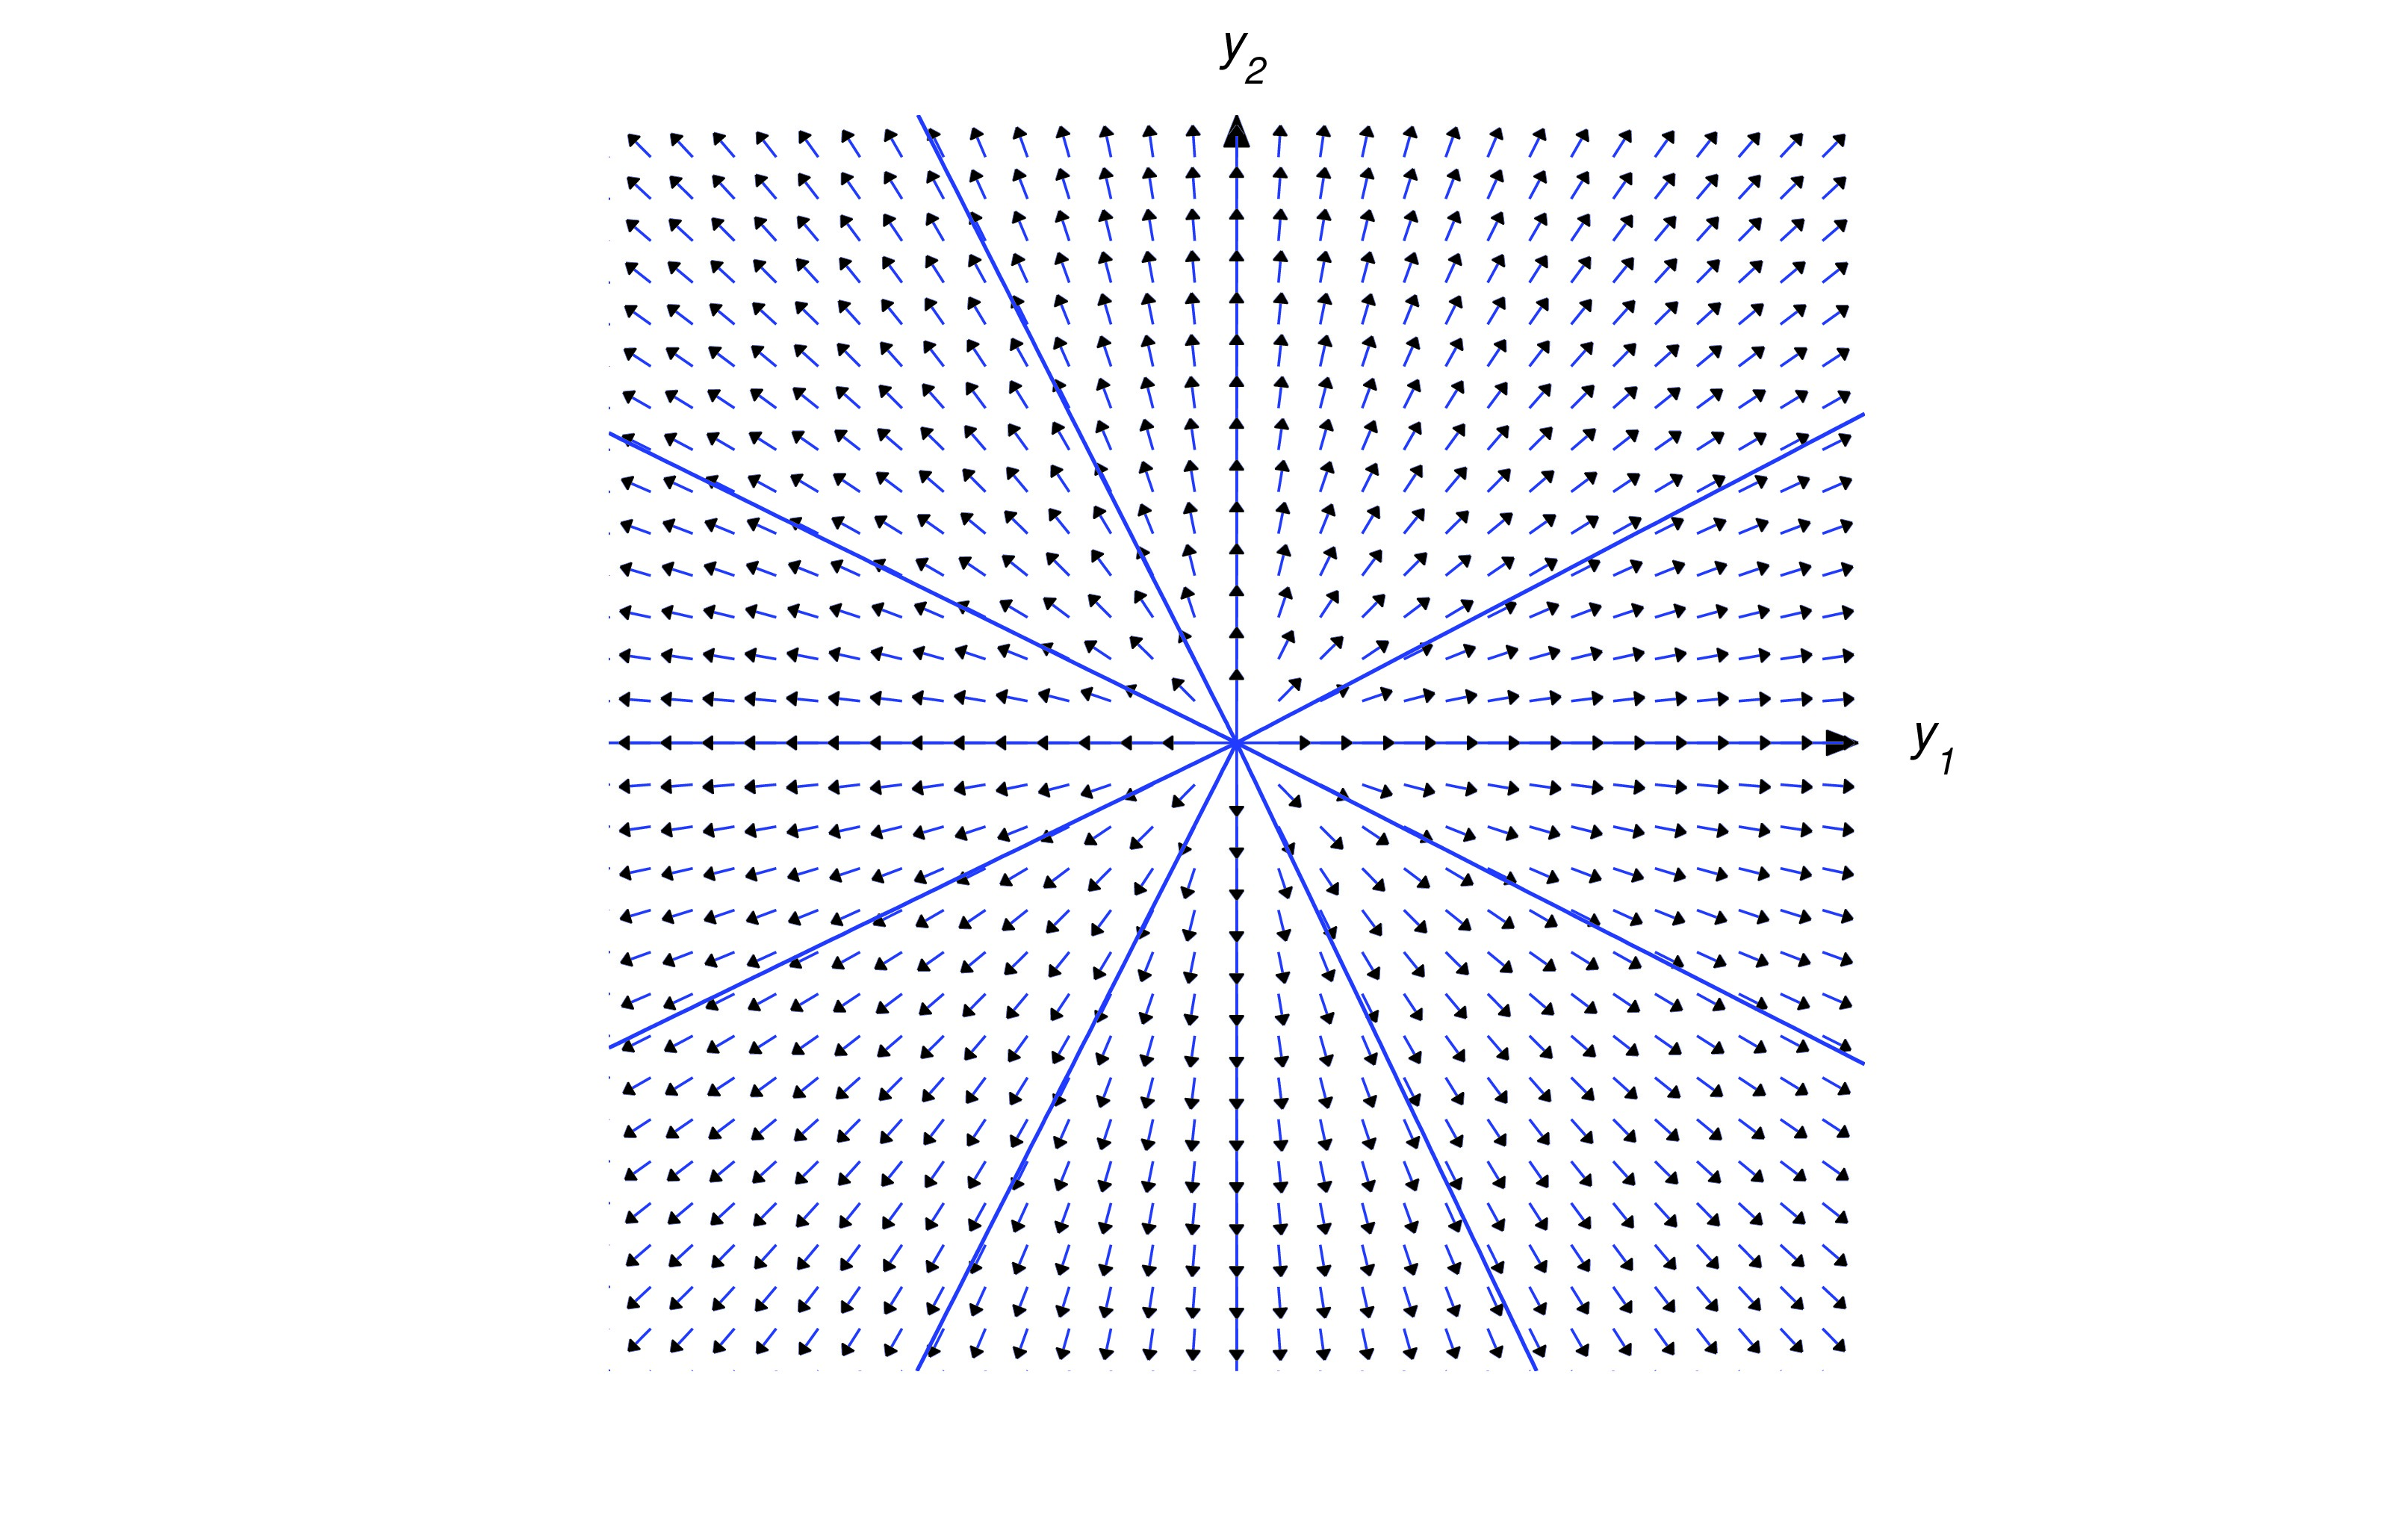
\includegraphics[height=1.5in]{fig100401.jpg} 
\end{image}


The direction of motion is toward the origin if $\lambda_1<0$, as shown in the figure. 
%(In these
%and the next figures an arrow through a point indicates the direction of motion along the trajectory through the point.)

\begin{image}
 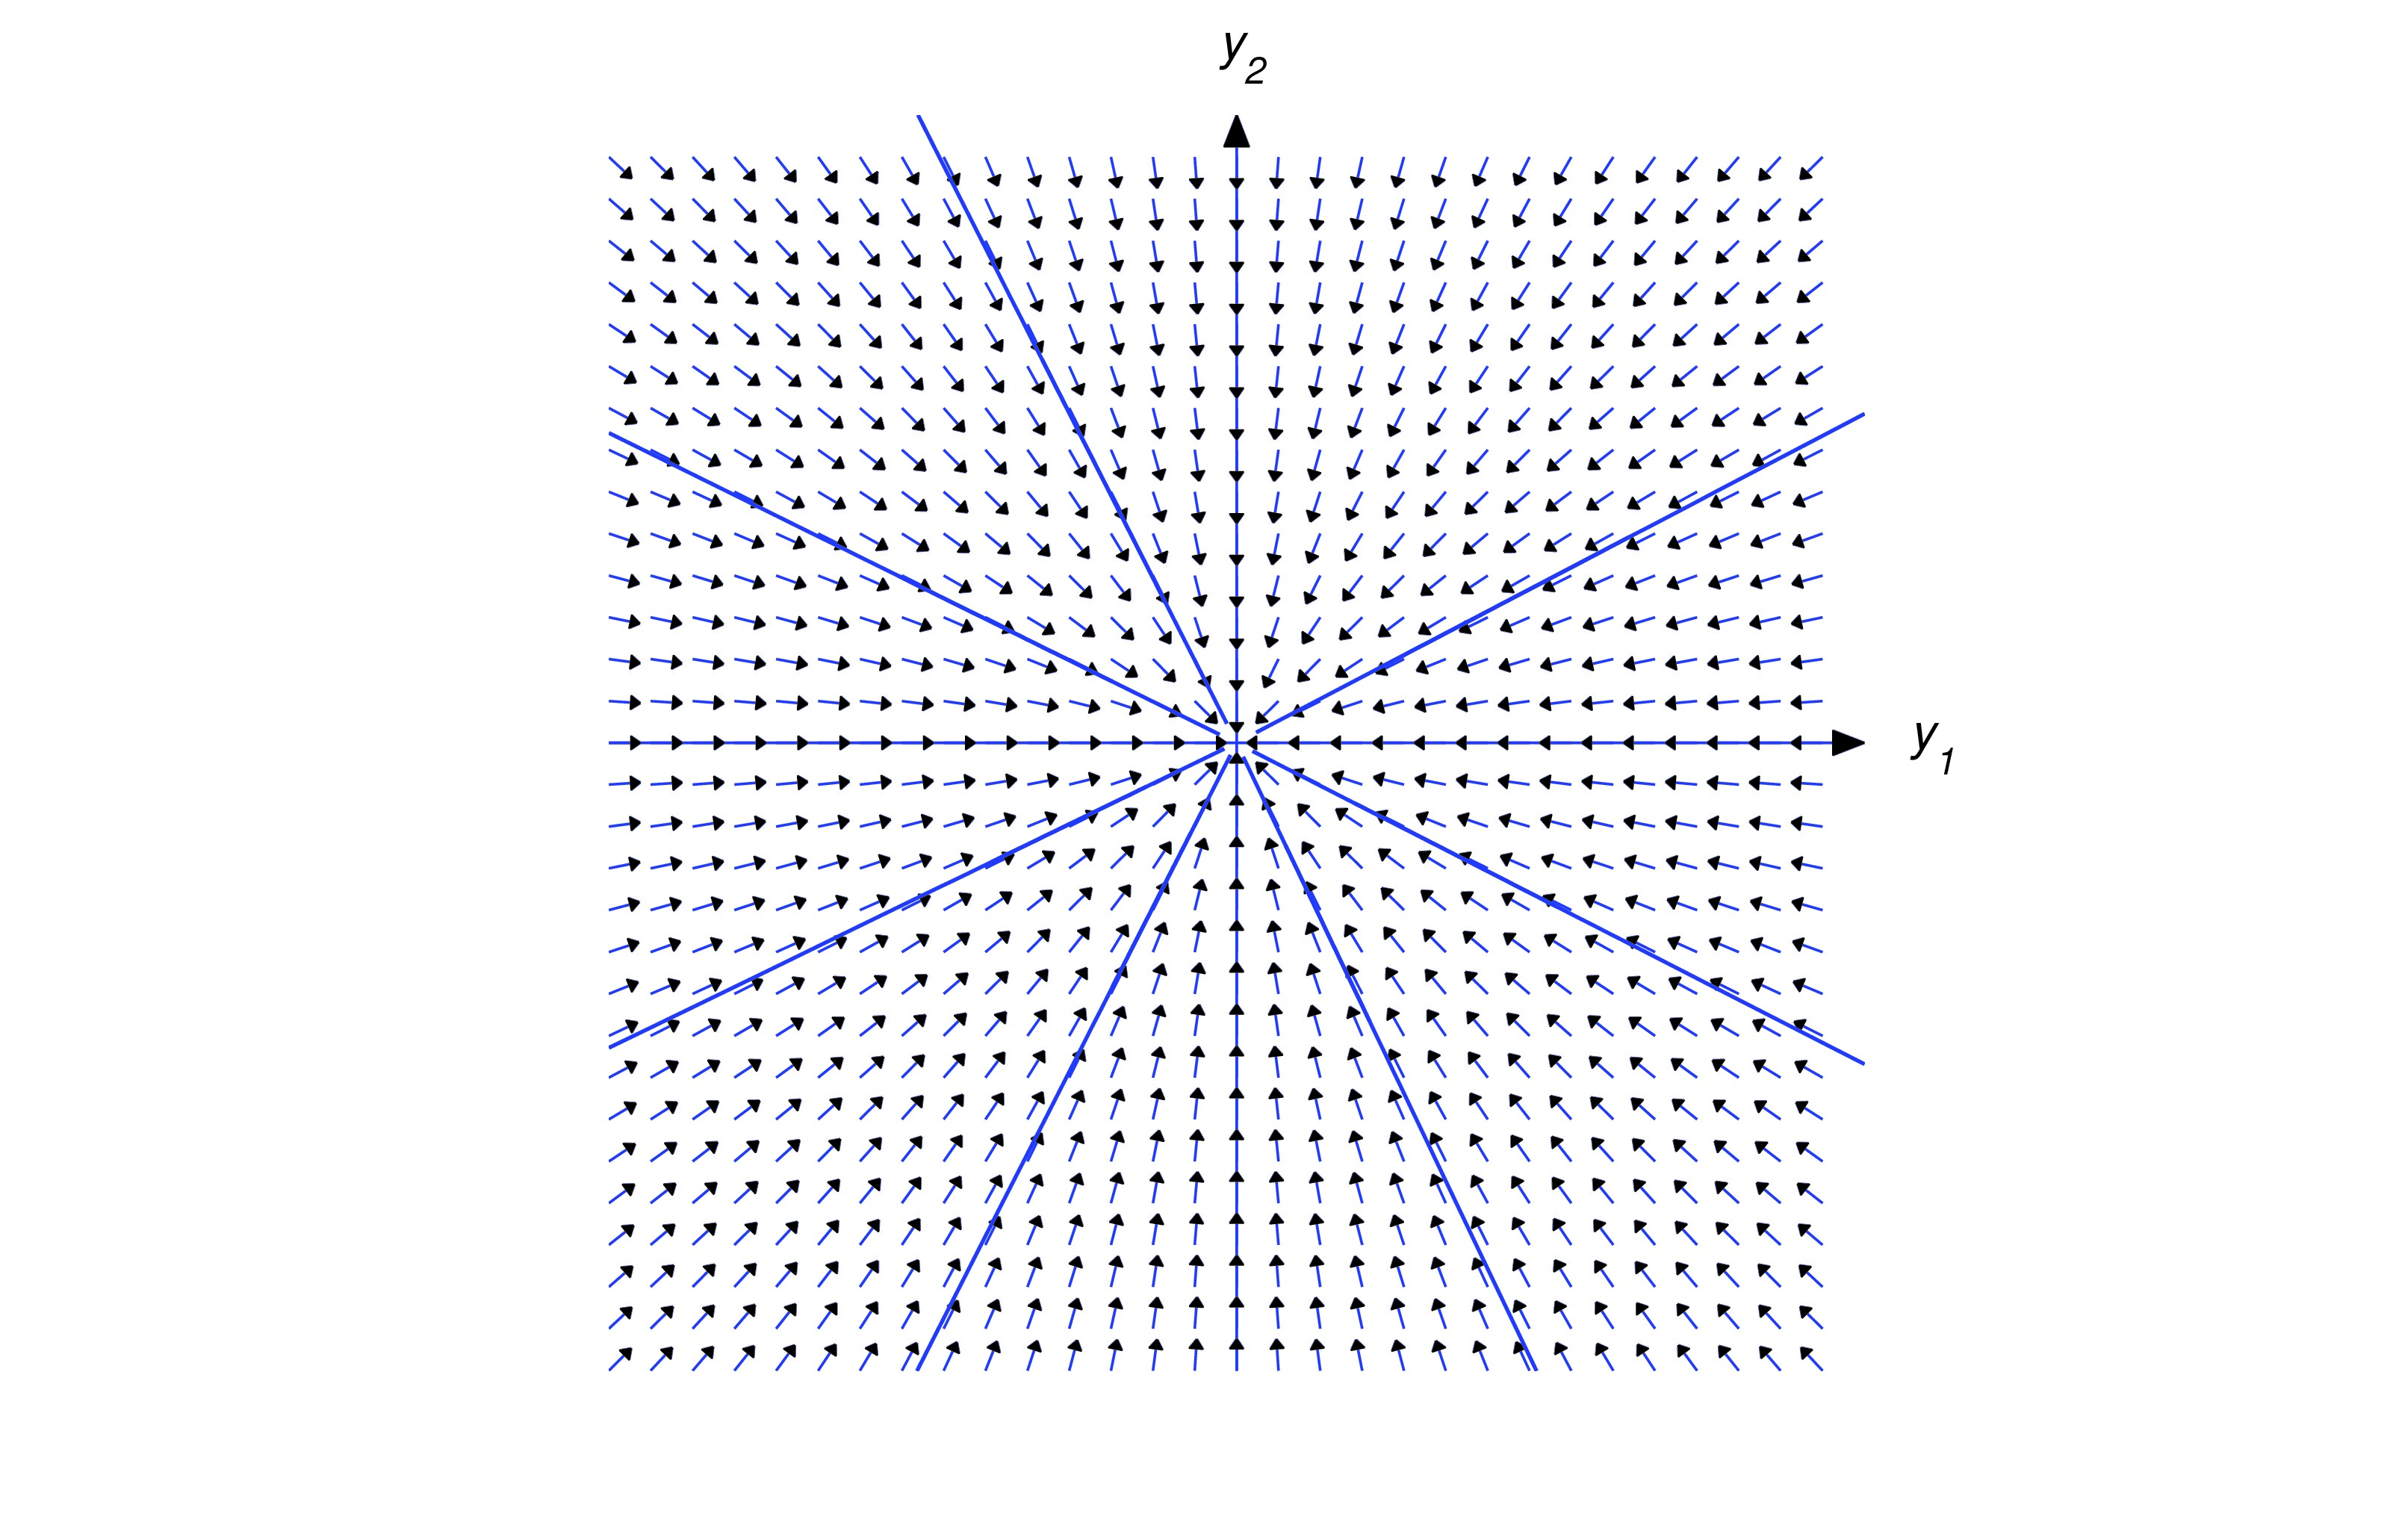
\includegraphics[height=1.5in]{fig100402.jpg} 
\end{image}

Now suppose   $\lambda_2>\lambda_1$, and let $L_1$ and $L_2$ denote
lines through the origin parallel to ${\bf x}_1$ and ${\bf x}_2$,
respectively. By a half-line of $L_1$ (or $L_2$), we mean either of the
rays obtained by removing the origin from $L_1$ (or $L_2$).

Letting $c_2=0$ in \eqref{eq:10.4.19} yields ${\bf y}=c_1{\bf
x}_1e^{\lambda_1 t}$. If $c_1\neq 0$, the trajectory defined by this
solution is a half-line of $L_1$. The direction of motion is away from
the origin if $\lambda_1>0$, toward the origin if $\lambda_1<0$.
Similarly, the trajectory of  ${\bf y}=c_2{\bf x}_2e^{\lambda_2 t}$
with $c_2\neq 0$ is a half-line of $L_2$.

Henceforth, we assume that $c_1$ and $c_2$ in \eqref{eq:10.4.19} are both
nonzero. In this case, the trajectory of \eqref{eq:10.4.19} can't
intersect
$L_1$ or $L_2$, since every point on these lines is on the trajectory
of a solution for which either $c_1=0$ or $c_2=0$. (Remember: distinct
trajectories can't intersect!). Therefore the trajectory of
\eqref{eq:10.4.19} must lie entirely in one of the four open sectors
bounded by $L_1$ and $L_2$, but do not any point  on $L_1$ or
$L_2$. Since the initial point $(y_1(0),y_2(0))$ defined by
$$
{\bf y}(0)=c_1{\bf x}_1+c_2{\bf x}_2
$$
is on the trajectory, we can determine which sector contains the
trajectory from the signs of $c_1$ and $c_2$,
as shown in the figure.

\begin{image}
 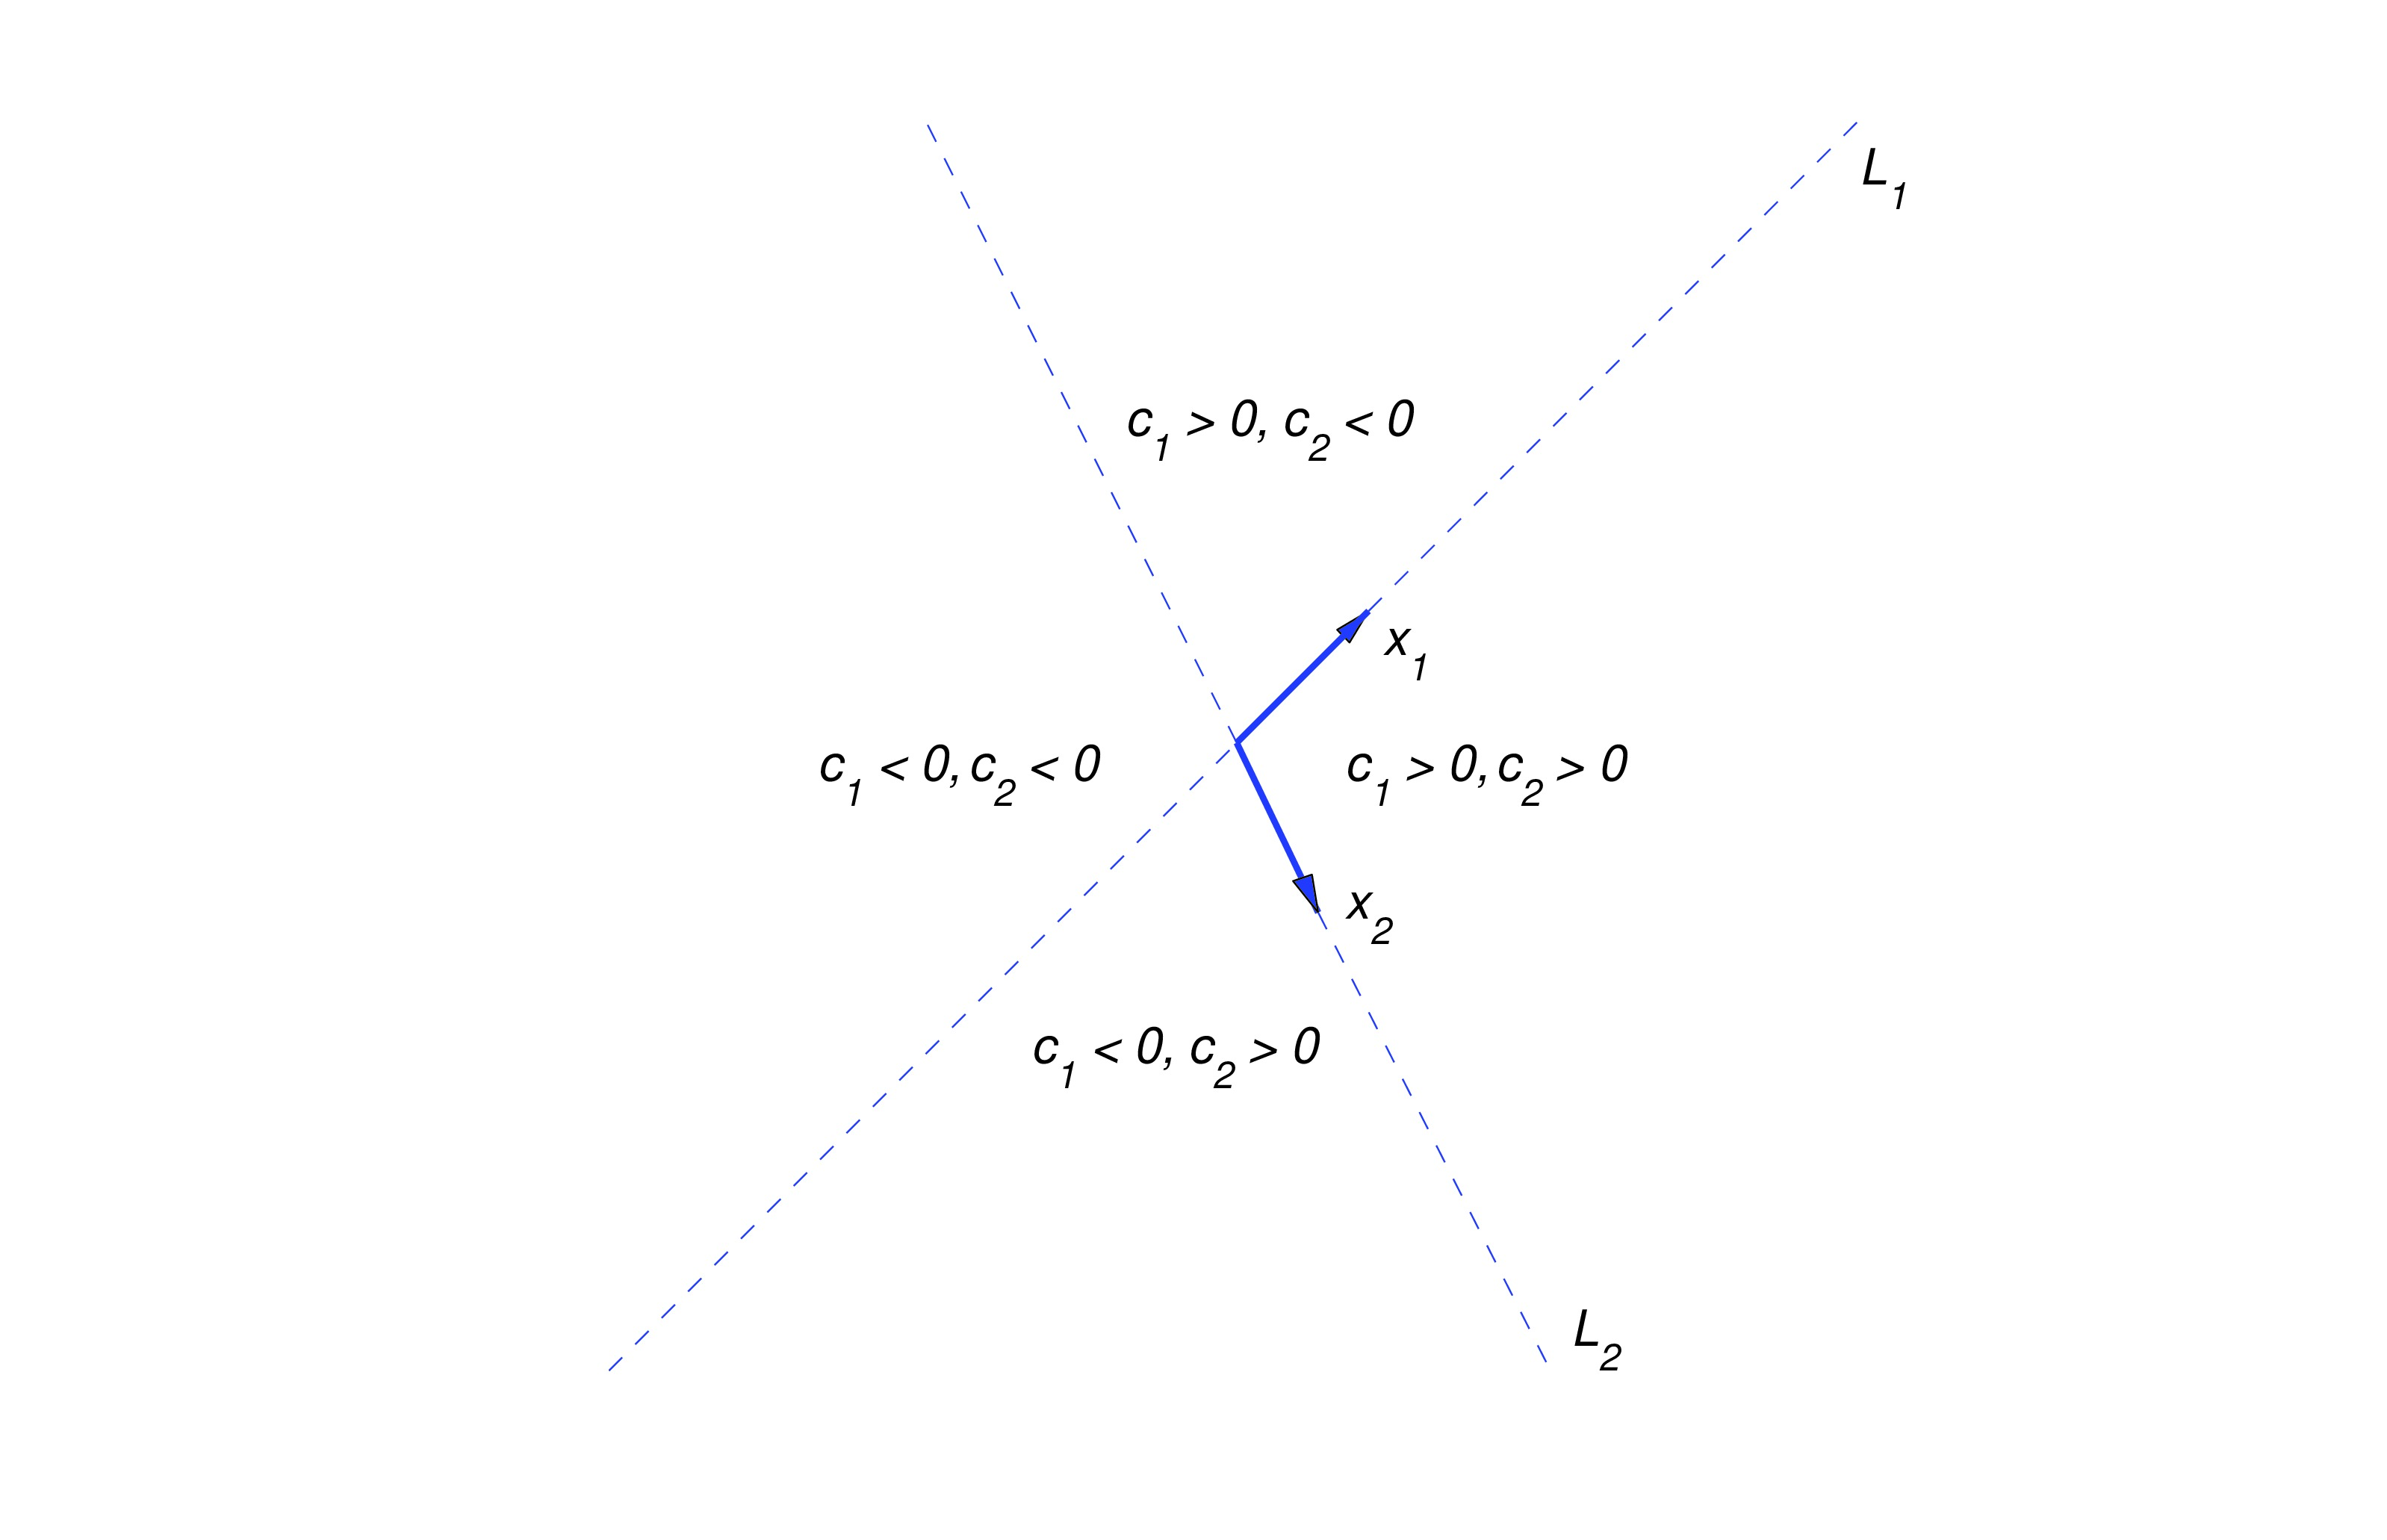
\includegraphics[height=1.5in]{fig100403.jpg} 
\end{image}

The direction of ${\bf y}(t)$ in \eqref{eq:10.4.19} is the
same as that of
\begin{equation} \label{eq:10.4.20}
e^{-\lambda_2 t}{\bf y}(t)=
c_1{\bf x}_1e^{-(\lambda_2-\lambda_1)t}+c_2{\bf x}_2
\end{equation}
and of
\begin{equation} \label{eq:10.4.21}
e^{-\lambda_1 t}{\bf y}(t)=c_1{\bf
x}_1+c_2{\bf x}_2e^{(\lambda_2-\lambda_1)t}.
\end{equation}
Since the right side of \eqref{eq:10.4.20} approaches $c_2{\bf x}_2$ as
$t\rightarrow\infty$, the trajectory is asymptotically parallel to $L_2$ as
$t\rightarrow\infty$. Since the right side of \eqref{eq:10.4.21} approaches
$c_1{\bf x}_1$ as $t\rightarrow-\infty$, the trajectory is asymptotically
parallel to $L_1$ as $t\rightarrow -\infty$.

The shape and direction of
traversal of the trajectory of \eqref{eq:10.4.19} depend upon whether
$\lambda_1$ and $\lambda_2$ are both positive, both negative, or of
opposite signs. We'll now analyze these three cases.

Henceforth $\norm{{\bf u}}$  denote the length of the vector
${\bf u}$.




{\bf Case 1:} $\lambda_2>\lambda_1>0$

The figure below  shows some
 typical trajectories.
 
 \begin{image}
 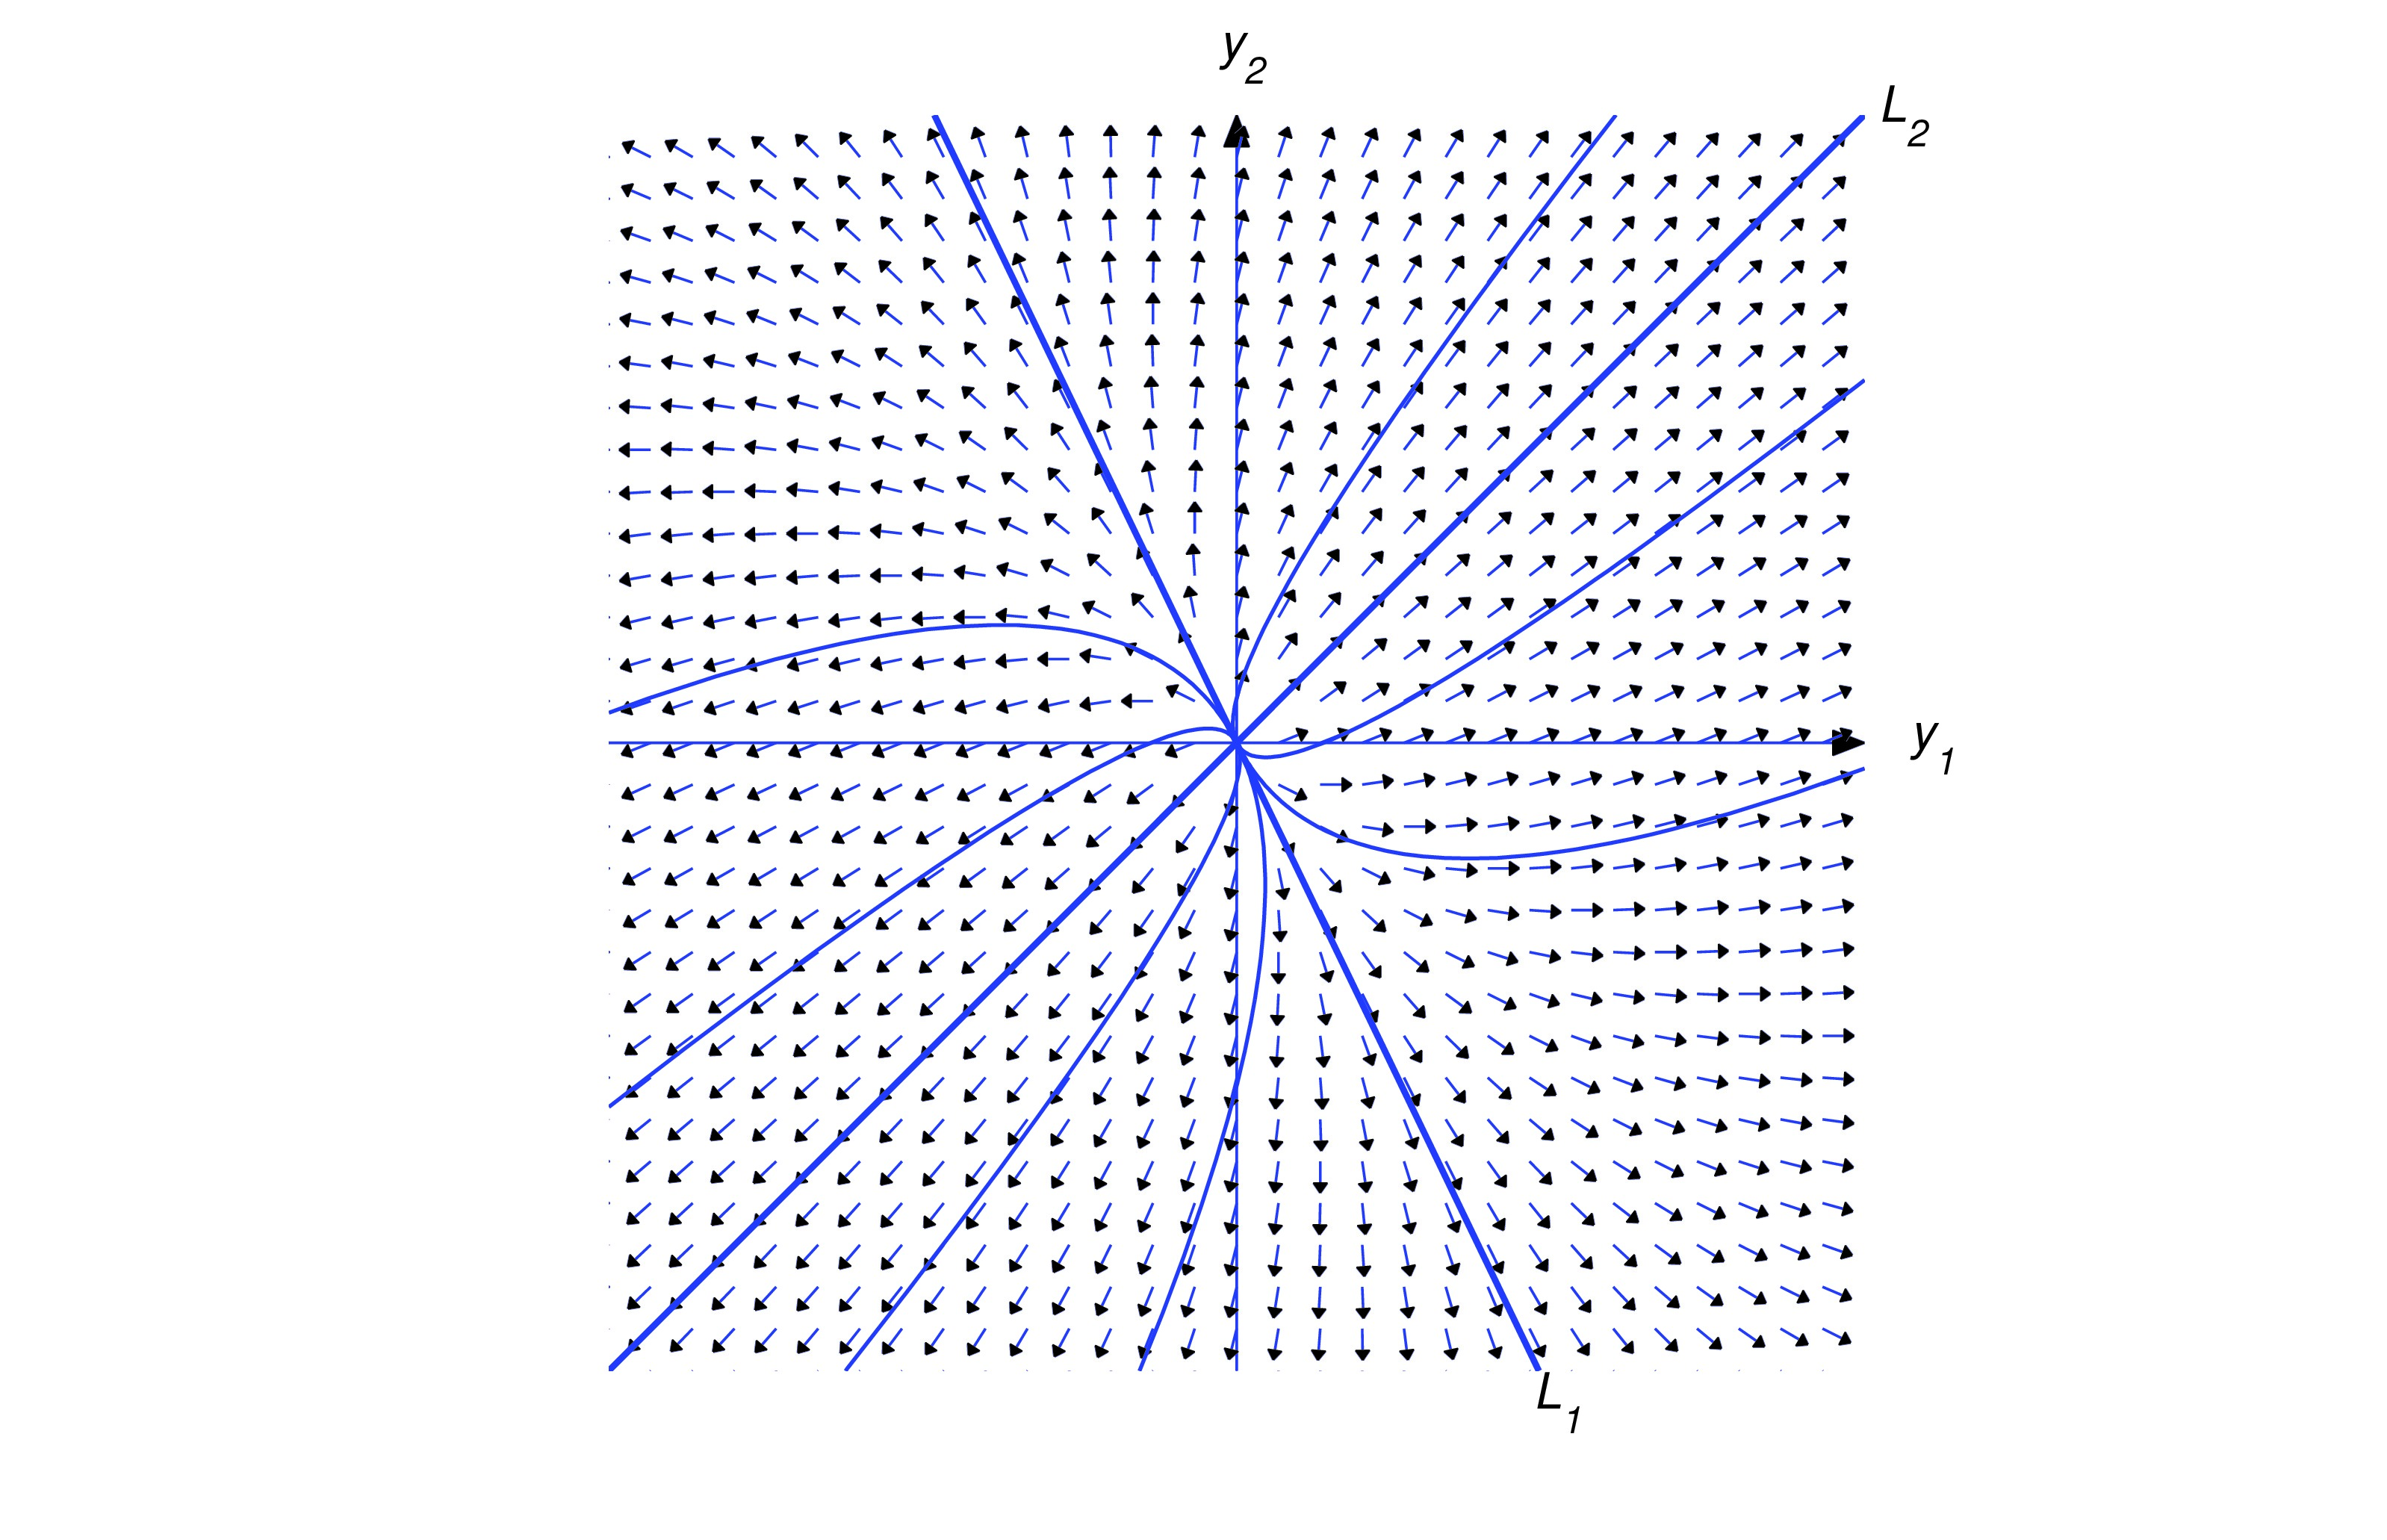
\includegraphics[height=1.5in]{fig100404.jpg} 
\end{image}
 
In this case, $\lim_{t\rightarrow -\infty}\norm{{\bf y}(t)}=0$, so the trajectory
is not only asymptotically parallel to $L_1$ as $t\rightarrow -\infty$, but is
actually asymptotically tangent to $L_1$ at the origin. On
the other hand, $\lim_{t\rightarrow\infty}\norm{{\bf y}(t)}=\infty$ and
$$
\lim_{t\rightarrow\infty}\norm{{\bf y}(t)-c_2{\bf x}_2e^{\lambda_2
t}}=\lim_{t\rightarrow\infty}\norm{c_1{\bf x_1}e^{\lambda_1t}}=\infty,
$$
so, although the trajectory is asymptotically parallel to $L_2$ as
$t\rightarrow\infty$, it's not asymptotically tangent to $L_2$.
The direction of motion along each trajectory is away from the origin.

{\bf Case 2:} $0>\lambda_2>\lambda_1$

The figure below shows
some typical trajectories.

\begin{image}
 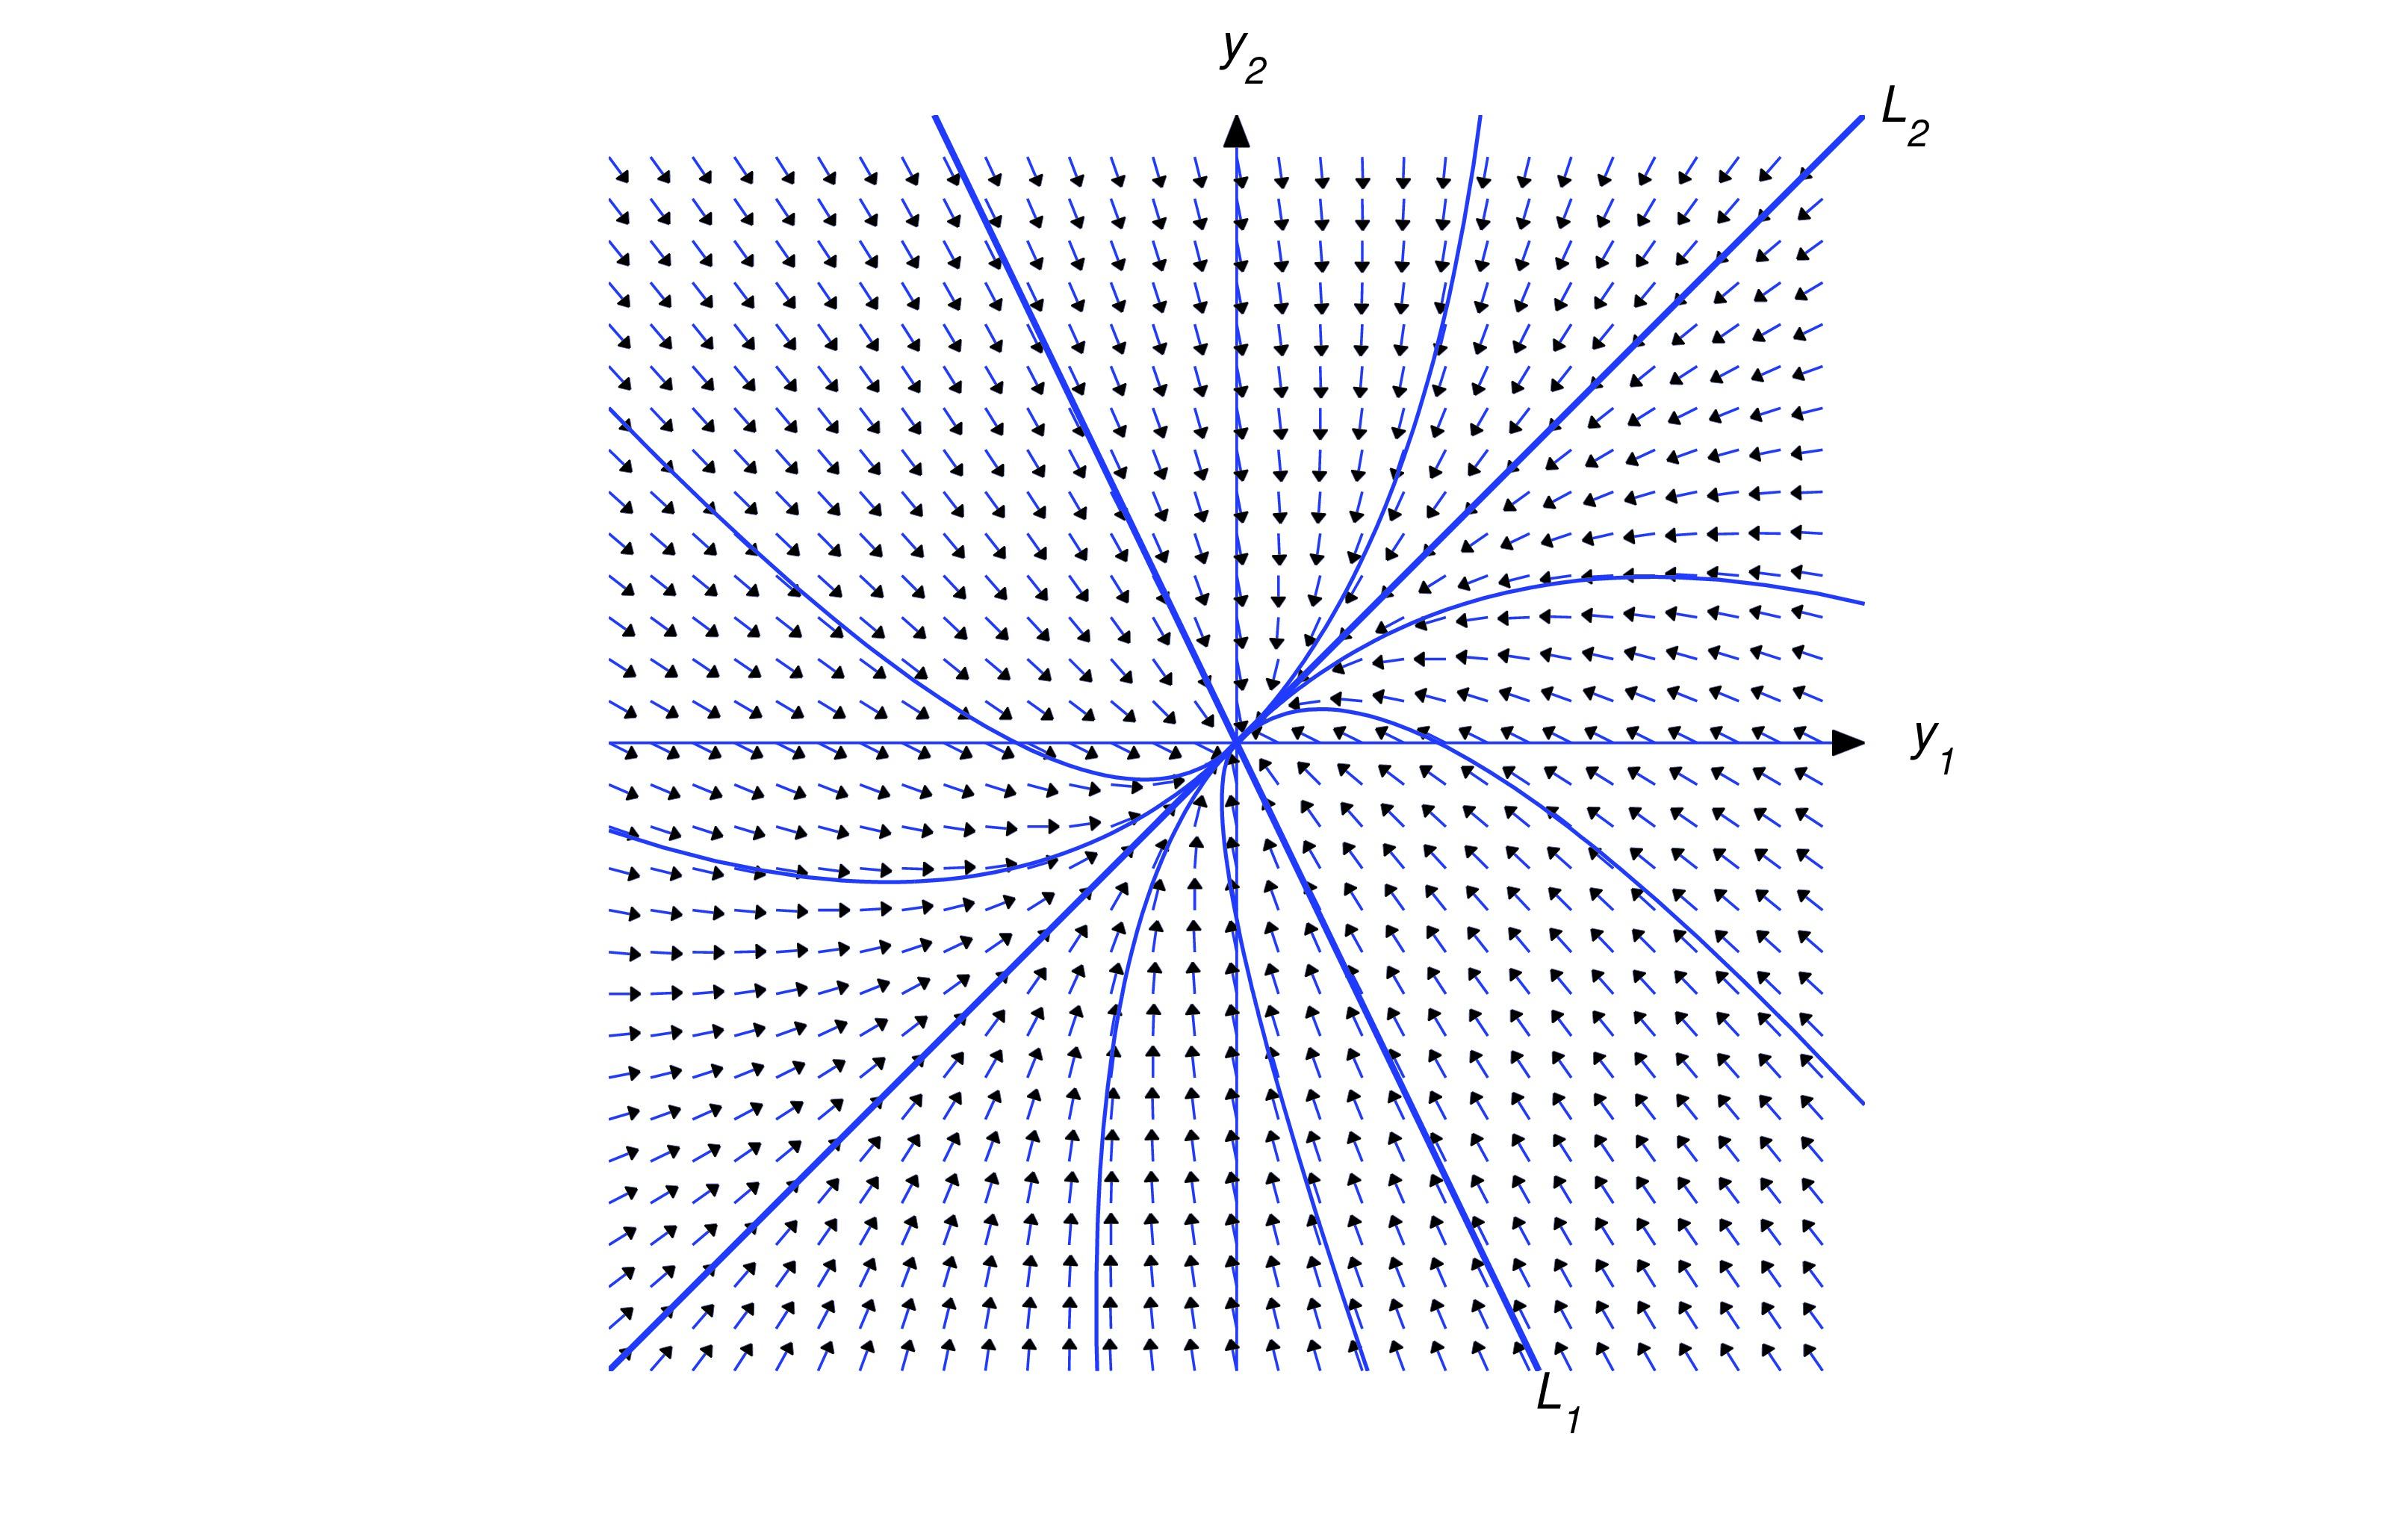
\includegraphics[height=1.5in]{fig100405.jpg} 
\end{image}

In this case, $\lim_{t\rightarrow\infty}\norm{{\bf y}(t)}=0$, so the trajectory is
asymptotically tangent to $L_2$ at the origin as $t\rightarrow\infty$. On the
other hand, $\lim_{t\rightarrow-\infty}\norm{{\bf y}(t)}=\infty$ and
$$
\lim_{t\rightarrow-\infty}\norm{{\bf y}(t)-c_1{\bf x}_1e^{\lambda_1
t}}=\lim_{t\rightarrow-\infty}\norm{c_2{\bf x}_2e^{\lambda_2t}}=\infty,
$$
so, although the trajectory is asymptotically parallel to $L_1$ as
$t\rightarrow-\infty$, it's not asymptotically tangent to it.
The direction of motion along each trajectory is toward the origin.

{\bf Case 3:} $\lambda_2>0>\lambda_1$

The figure below shows
some typical trajectories.

\begin{image}
 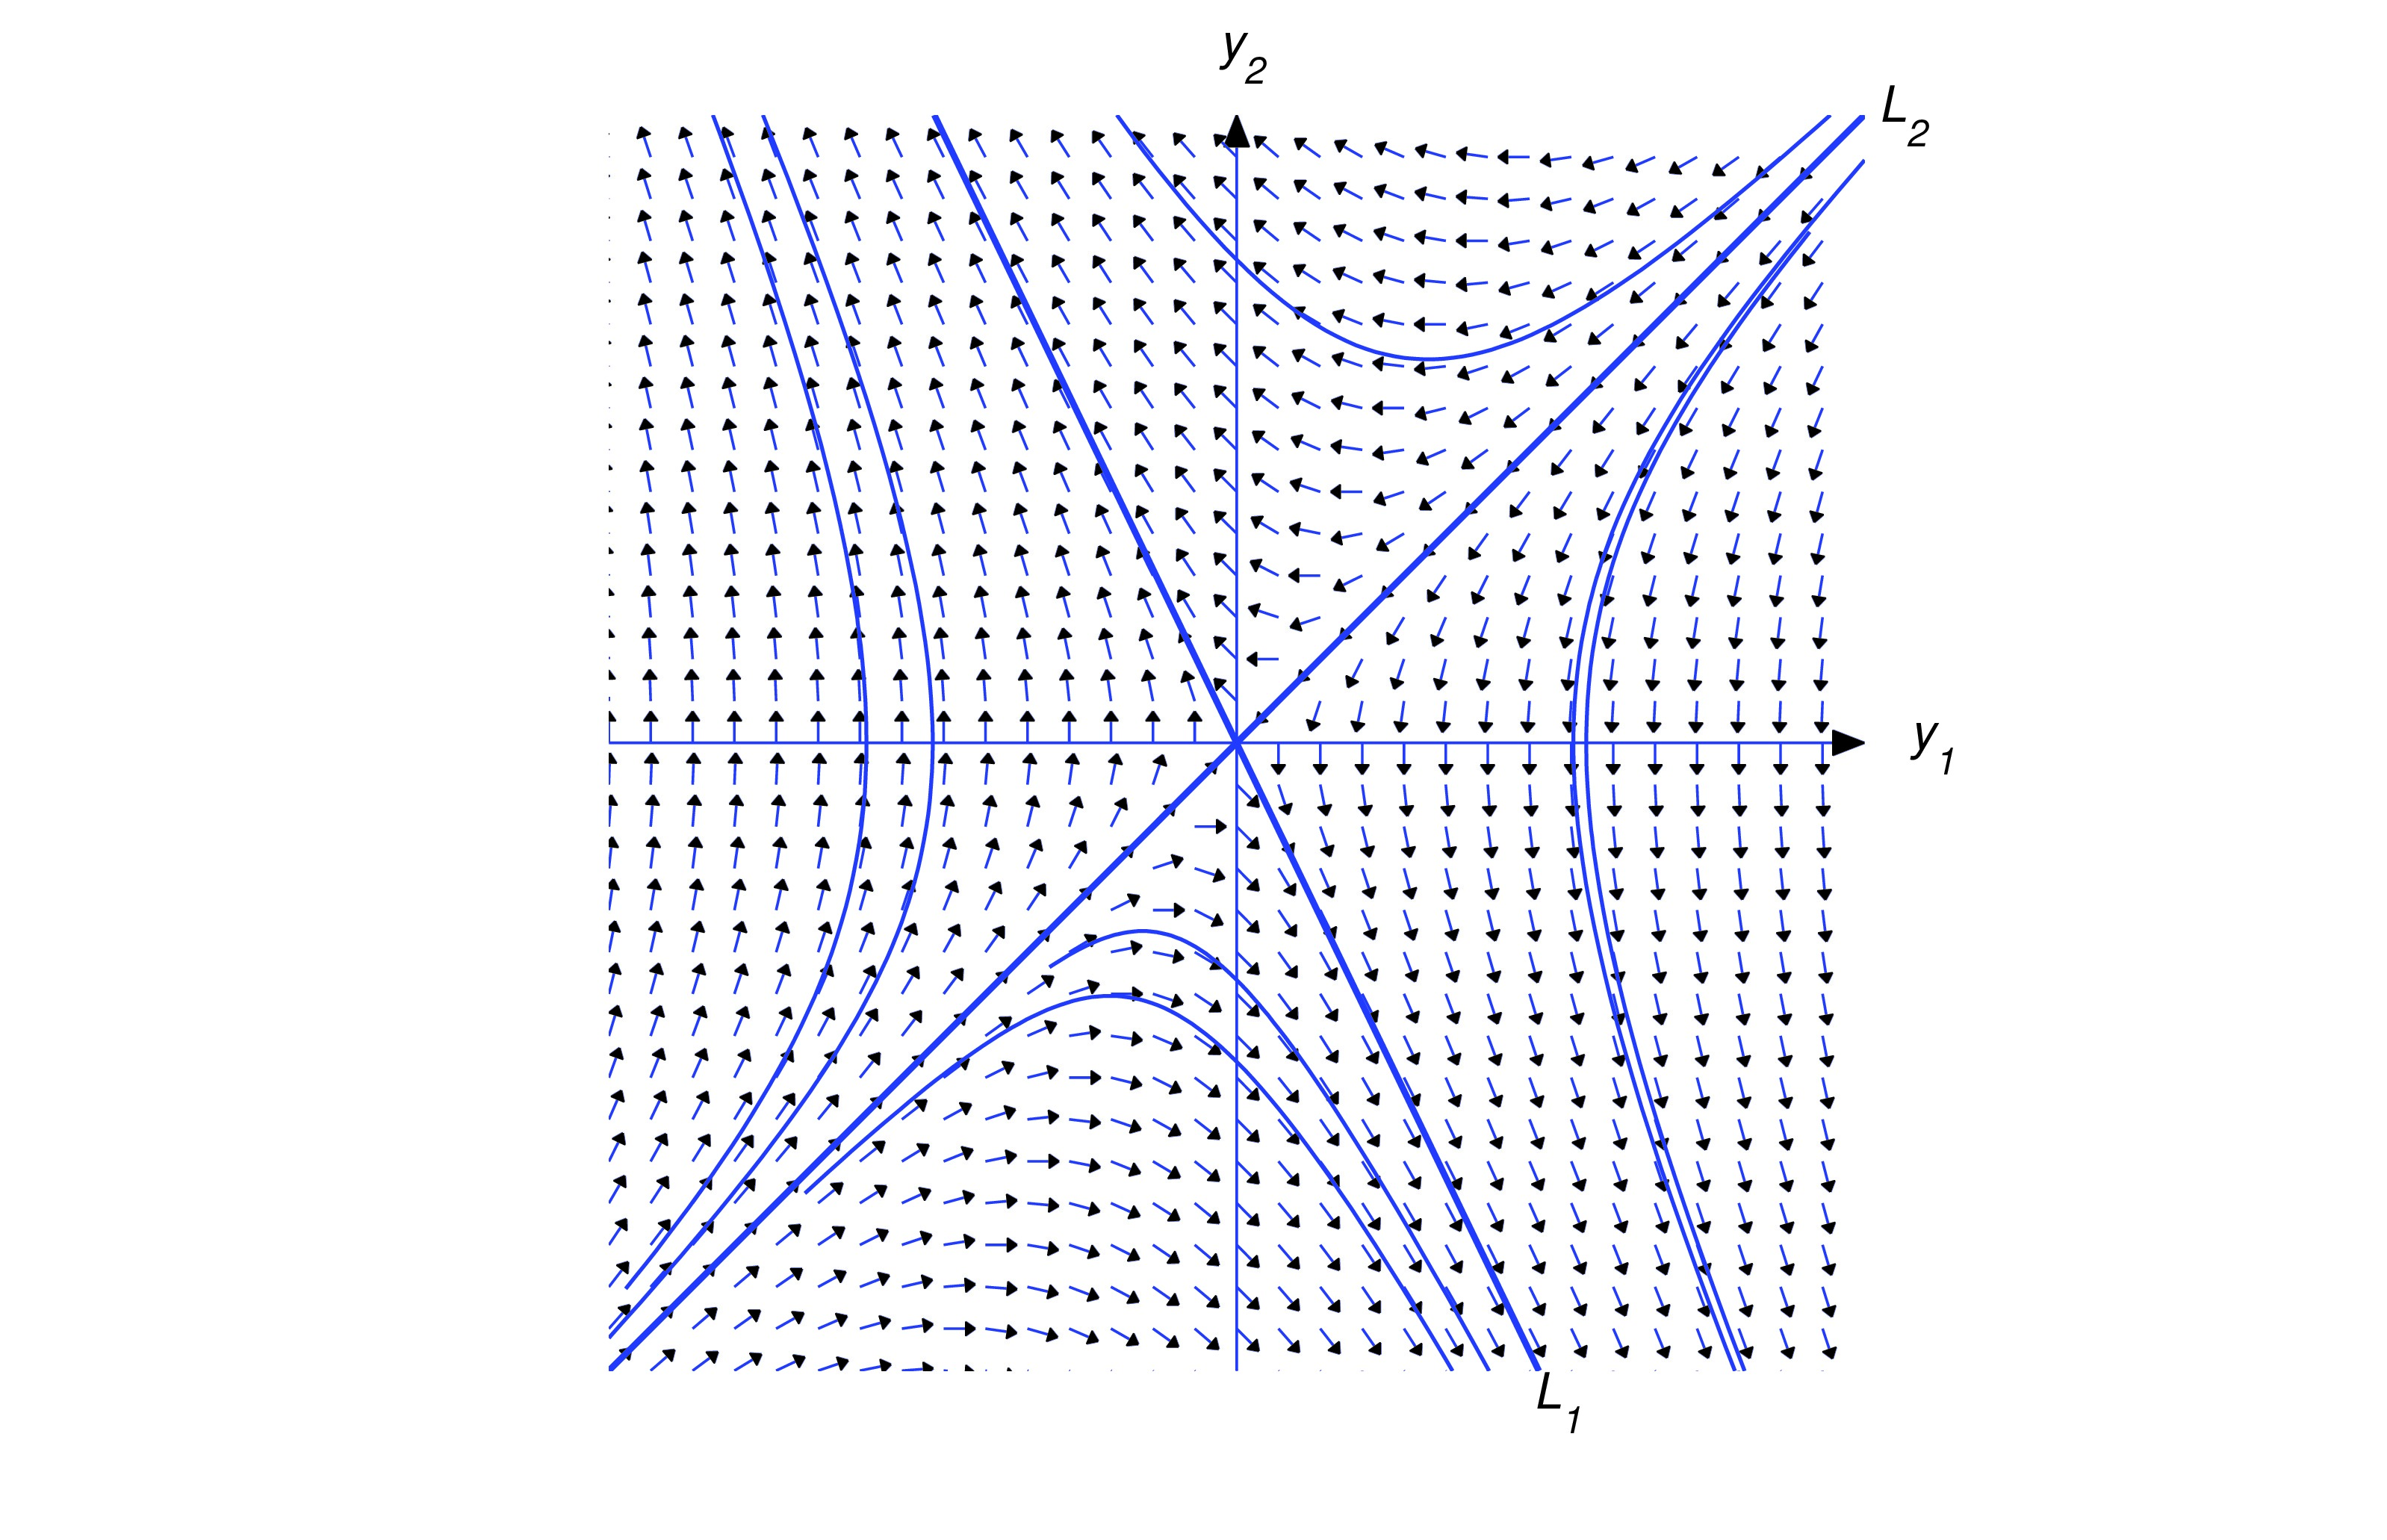
\includegraphics[height=1.5in]{fig100406.jpg} 
\end{image}

In this case,
$$
\lim_{t\rightarrow\infty}\norm{{\bf y}(t)}=\infty \quad\mbox{and}\quad
\lim_{t\rightarrow\infty}\norm{{\bf y}(t)-c_2{\bf x}_2e^{\lambda_2
t}}=\lim_{t\rightarrow\infty}\norm{c_1{\bf x}_1e^{\lambda_1t}}=0,
$$
so the trajectory is asymptotically tangent to $L_2$ as $t\rightarrow\infty$.
Similarly,
$$
\lim_{t\rightarrow -\infty}\norm{{\bf y}(t)}=\infty \quad\mbox{and}\quad
\lim_{t\rightarrow -\infty}\norm{{\bf y}(t)-c_1{\bf x}_1e^{\lambda_1
t}}=\lim_{t\rightarrow -\infty}\norm{c_2{\bf x}_2e^{\lambda_2t}}=0,
$$
so the trajectory is asymptotically tangent to $L_1$ as $t\rightarrow-\infty$.
The direction of motion is toward the origin on $L_1$ and away from
the origin on $L_2$. The direction of motion along any other
trajectory is away from $L_1$, toward $L_2$.




\section*{Text Source}
Trench, William F., "Elementary Differential Equations" (2013). Faculty Authored and Edited Books \& CDs. 8. (CC-BY-NC-SA)

\href{https://digitalcommons.trinity.edu/mono/8/}{https://digitalcommons.trinity.edu/mono/8/}


\end{document}